\graphicspath{{Figures/Dataset_Selection_Cuts/}}


\section{\label{Data}Dataset, event and track selections}


\subsection{\label{Data}Data sample}

\paragraph{Run}
The $\Upsilon$ analysis presented in this note is based on the first ALICE \PbPb\sep data taking of the LHC run 2 at a center of mass energy \sqrtSnnE{5.02} which took place in November-December 2015.
A full description of the ALICE detectors can be found in \cite{ALICEexpe}.
The present study is performed on the AOD175, officially produced from the muon\_calo\_pass1 reconstruction of the LHC15o period including the latest alignement configuration, by analyzing the reconstructed tracks in the muon spectrometer apparatus.
A detailed description of the muon reconstruction algorithm is given in \cite{simuSpectro, LongJpsiPaper}.
A total of 137 runs pass the quality assurance checks (QA). 
The {QA Muon} report of this period can be found \href{https://twiki.cern.ch/twiki/bin/view/ALICE/MuonPbPbQA2015}{here}.


\paragraph{\label{Event}Event selection}
The dataset analyzed is based on the dimuon events triggered by the muon spectormeter. 
More details can be found in \cite{LongJpsiPaper,UpsilonPbPb276ALICE}.
A logical OR of {CMUL7-B-NOPF-MUFAST} (unlike sign dimuon low \pt threshold) and {CMLL7-B-NOPF-MUFAST} (like sign dimuon low \pt threshold) trigger classes is used to filter the dimuon events.
The like sign dimuons are selected in order to perform the event mixing procedure (normalization method \ref{mixing}) as well as the {CMSL-B-NOPF-MUFAST} (single muon low \pt threshold).
In order to reject the beam-gas and debunched collisions the physics selection cuts are applied. 
The remaining dataset is then filtered to select events which are within the centrality class of $0-90\%$.
More details on the centrality estimation can be found \href{https://twiki.cern.ch/twiki/bin/view/ALICE/CentralityCodeSnippets#Anchor_Point}{here}.


\subsection{\label{TrackCut}Track and pair selection}

In order to clean the dataset of tracks with the aim of forming the opposite sign dimuon invariant mass spectrum we require that the following conditions are satisfied for each tracks and pairs:

\paragraph{track cuts}
\begin{itemize}
\item $-4.0<\eta<-2.5$  to reject tracks at the edges of the spectrometer acceptance,
\item $17.6<R_{\rm abs}<89.5$ to remove tracks crossing the thicker part of the front absorber,
\item matching between a reconstructed trigger track passing the hardware Low $p_{\rm T}$ threshold ($\pttrig>1$ GeV/$c$) and a reconstructed tracker track,
\item $p$DCA: product of the track momentum $p$ by the distance of the extrapolated track to the transverse plane containing the vertex DCA (Distance of Closest Approach). 
This selection remove the fake tracks (tracks which do not point to the vertex) present essentially in central collisions.
A cut has been tuned on data and set to $6\times\sigma_{p\rm DCA}$, where $\sigma_{p\rm DCA}$ is the resolution of this quantity.
\item $p_{\rm T}>2$ GeV/$c$: this selection reduces significantly the combinatorial background by increasing the significance of the signal.
A study has been performed on the embedding MC production.
The distributions of the opposite sign dimuon identified as background (left) and as \ups embedded signal (right), after applying all the previous track cuts including $p$DCA, are represented on the figure \ref{sigbkg} as a function of the \pt of each muon according to their sign.
A cut at 2 GeV/$c$ has been chosen as in previous \upsi analyses.
The evolution of the significance as a function of the \pt cut applied on each muons can be observed on the figure \ref{signifi}.
The maximum of significance is find for $\pt^{\mu^{+}}=\pt^{\mu^{-}}=2.5$\;GeV/$c$.
Nevertheless, the increase of significance in raw data by applying a muon \pt cut of 2.5\;GeV/$c$ with respect 2\;GeV/$c$ is negligible.
Furthermore, a muon \pt cut at 2\;GeV/$c$ remove almost  no \ups signal ($<1\%$).
Thus none systematic uncertainty has been assigned to this track cut.
\end{itemize}

\begin{figure}[!t]
\begin{center}
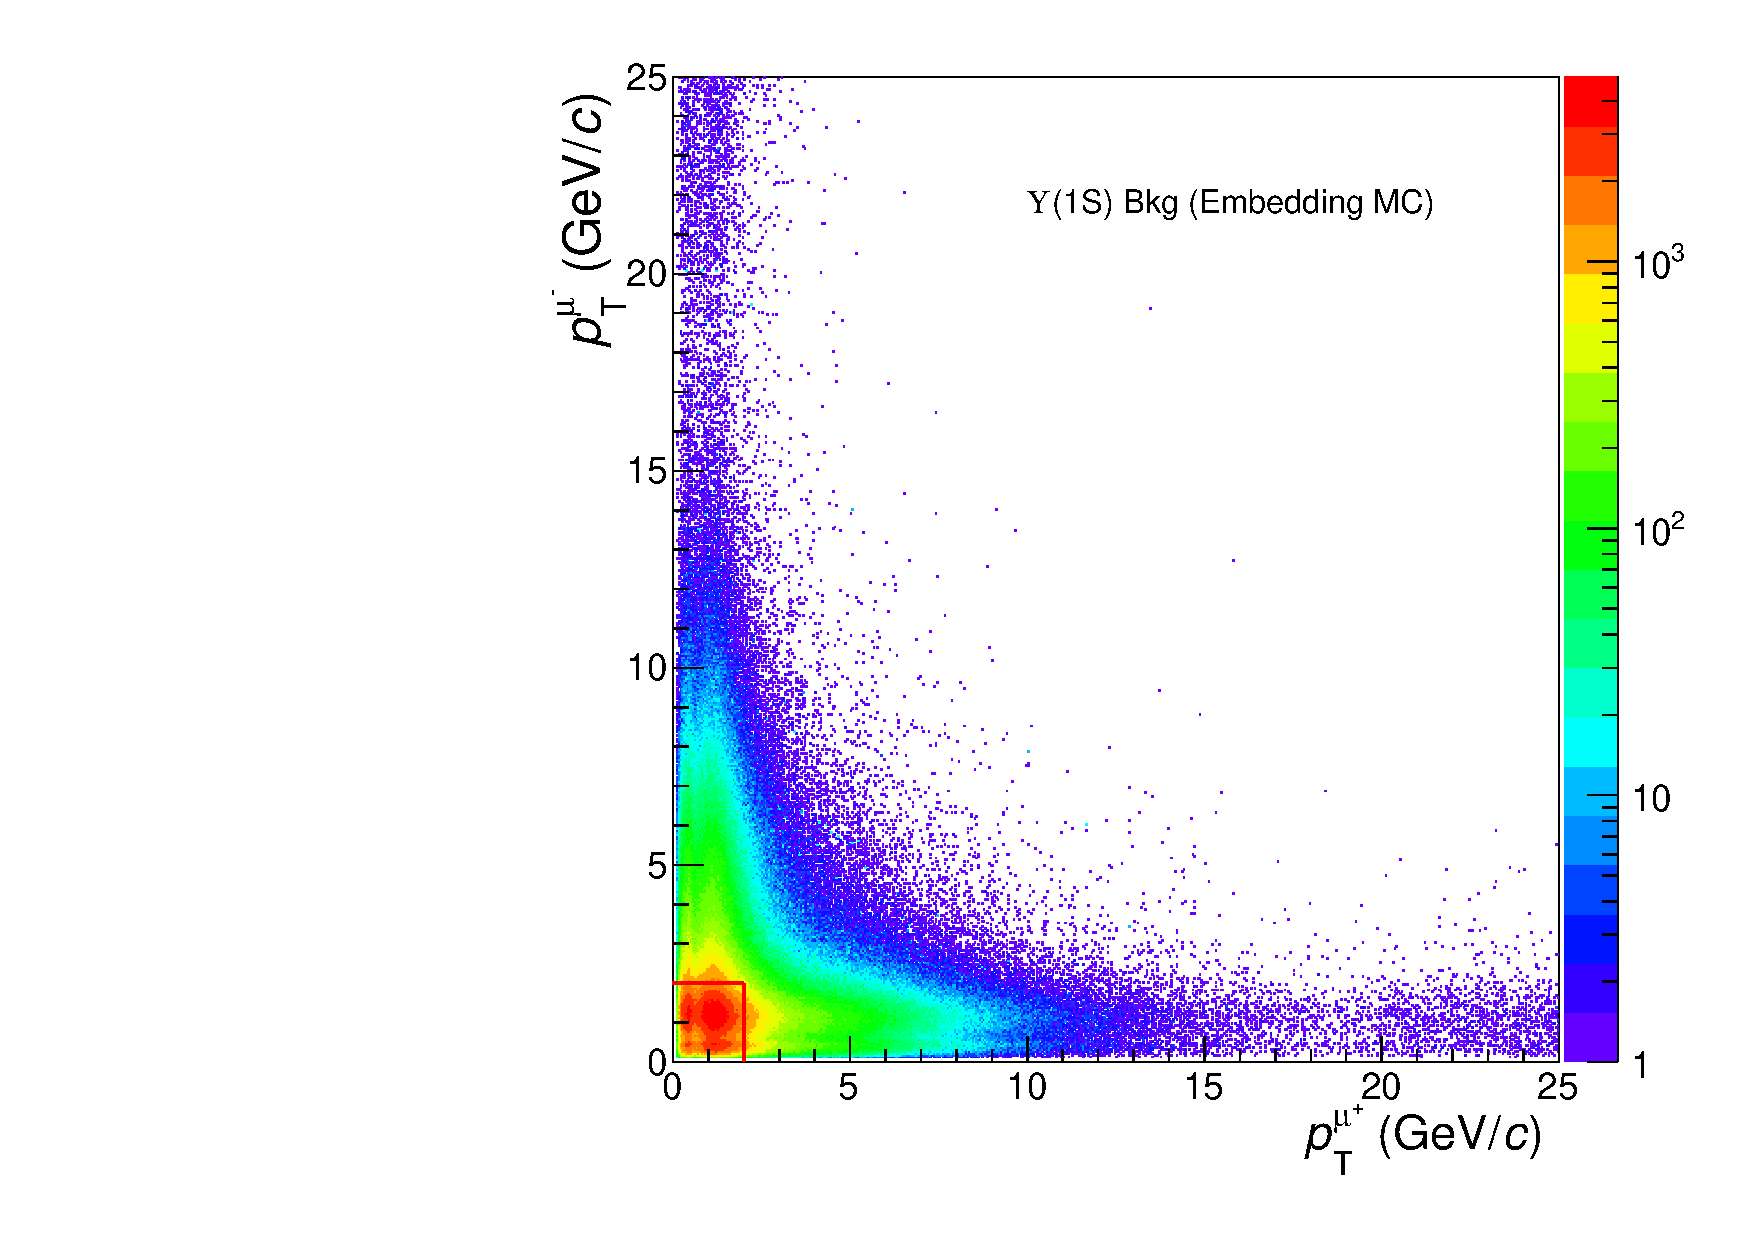
\includegraphics[width=6cm]{MuonPtCut/background.pdf}
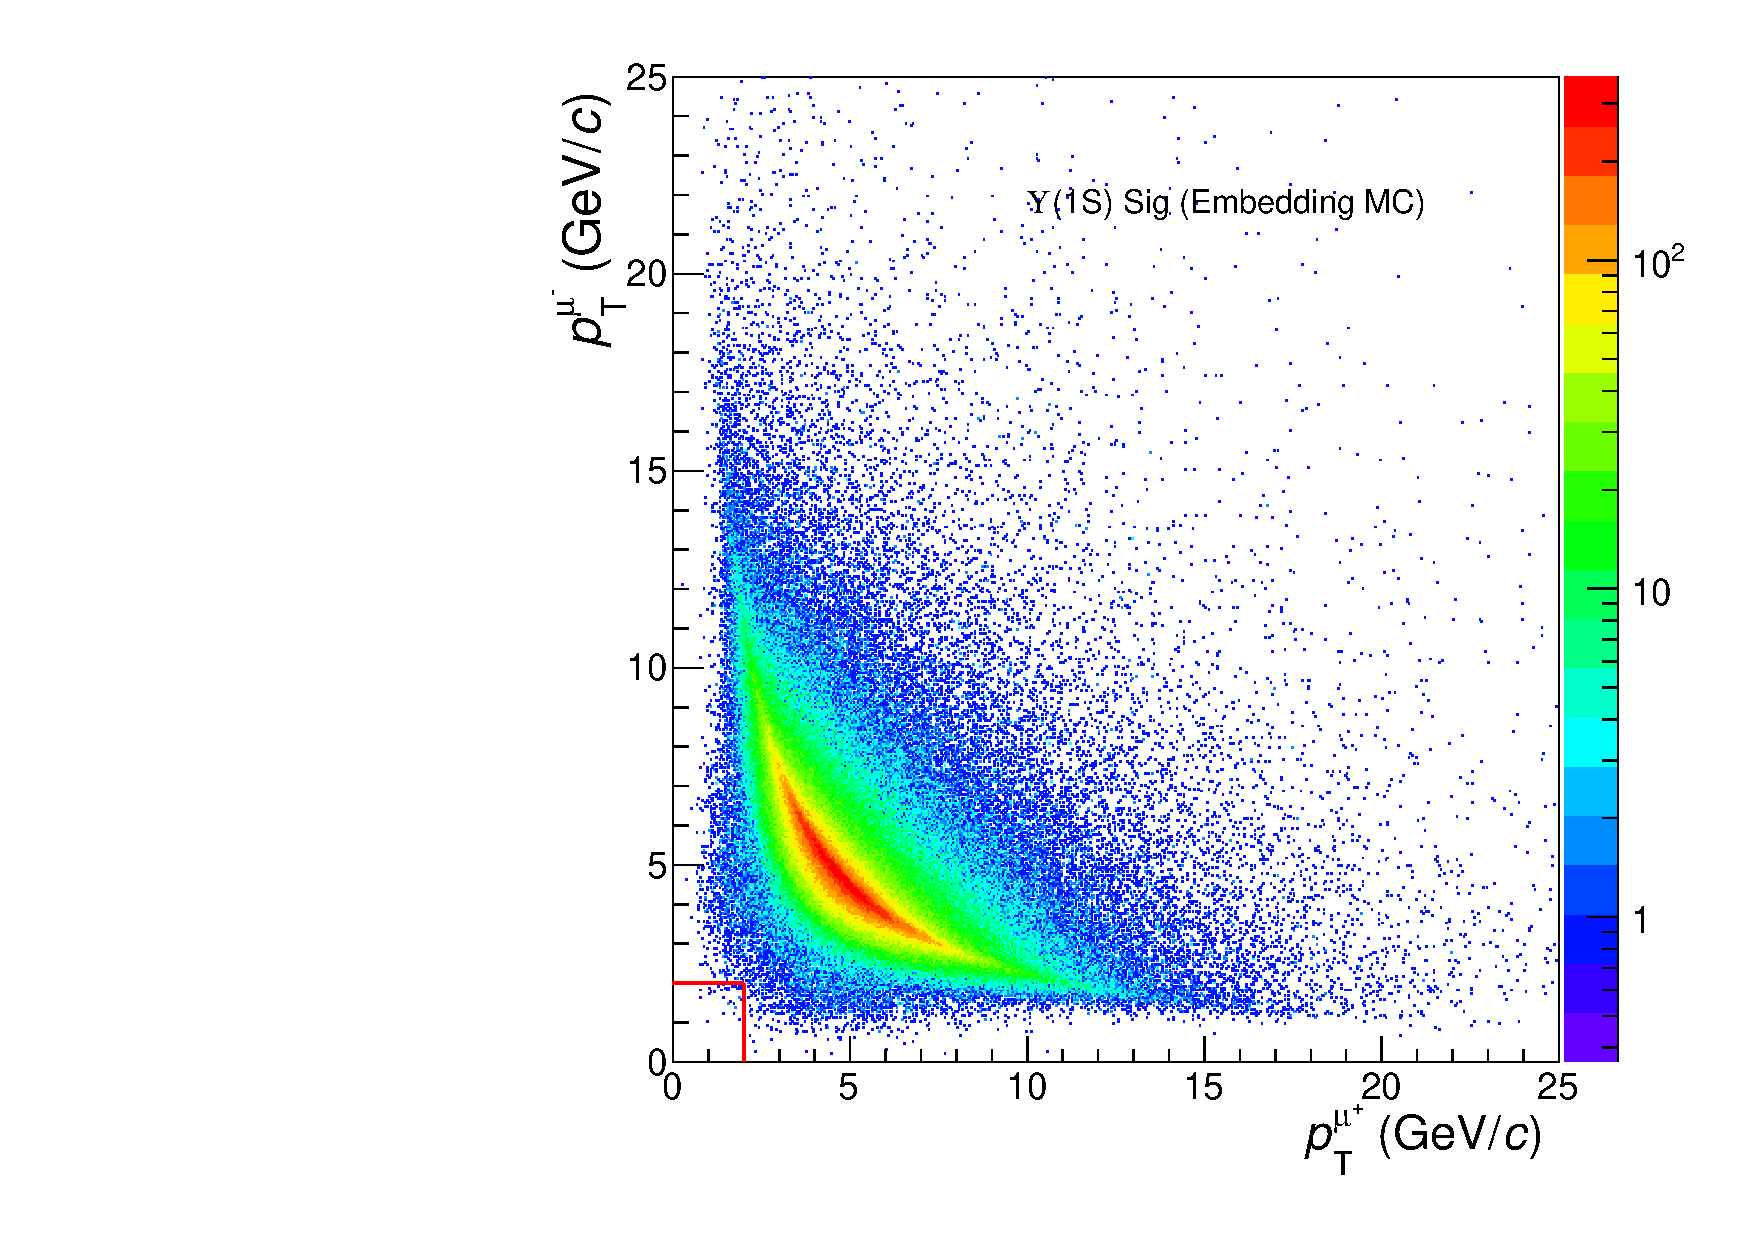
\includegraphics[width=6cm]{MuonPtCut/signal.pdf}
\end{center}
\caption{\label{sigbkg}Background (left) and \ups signal (right) distributions as a function of the \pt of each muon extracted from embedding MC.}
\end{figure}

\begin{figure}[!t]
\begin{center}
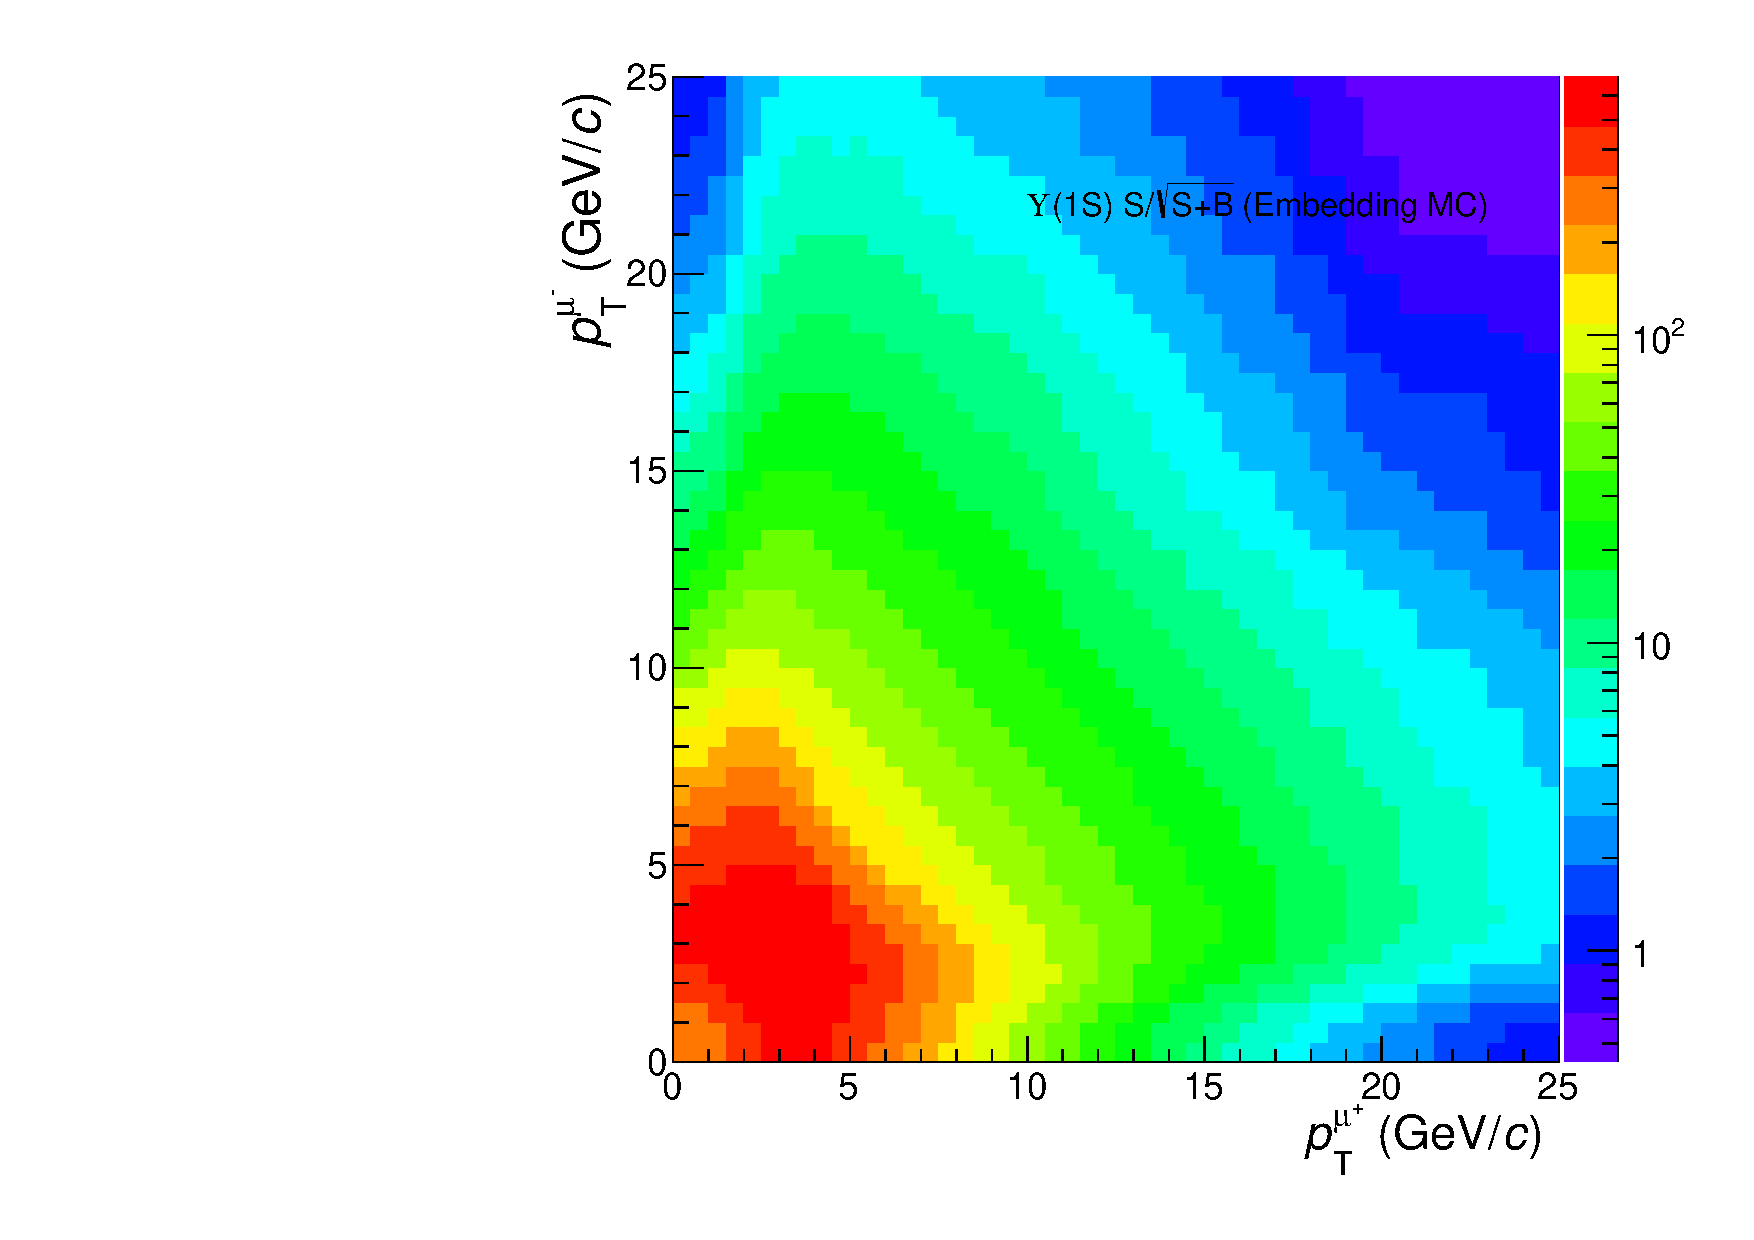
\includegraphics[width=6cm]{MuonPtCut/significance_rebin10_ptmax25.pdf}
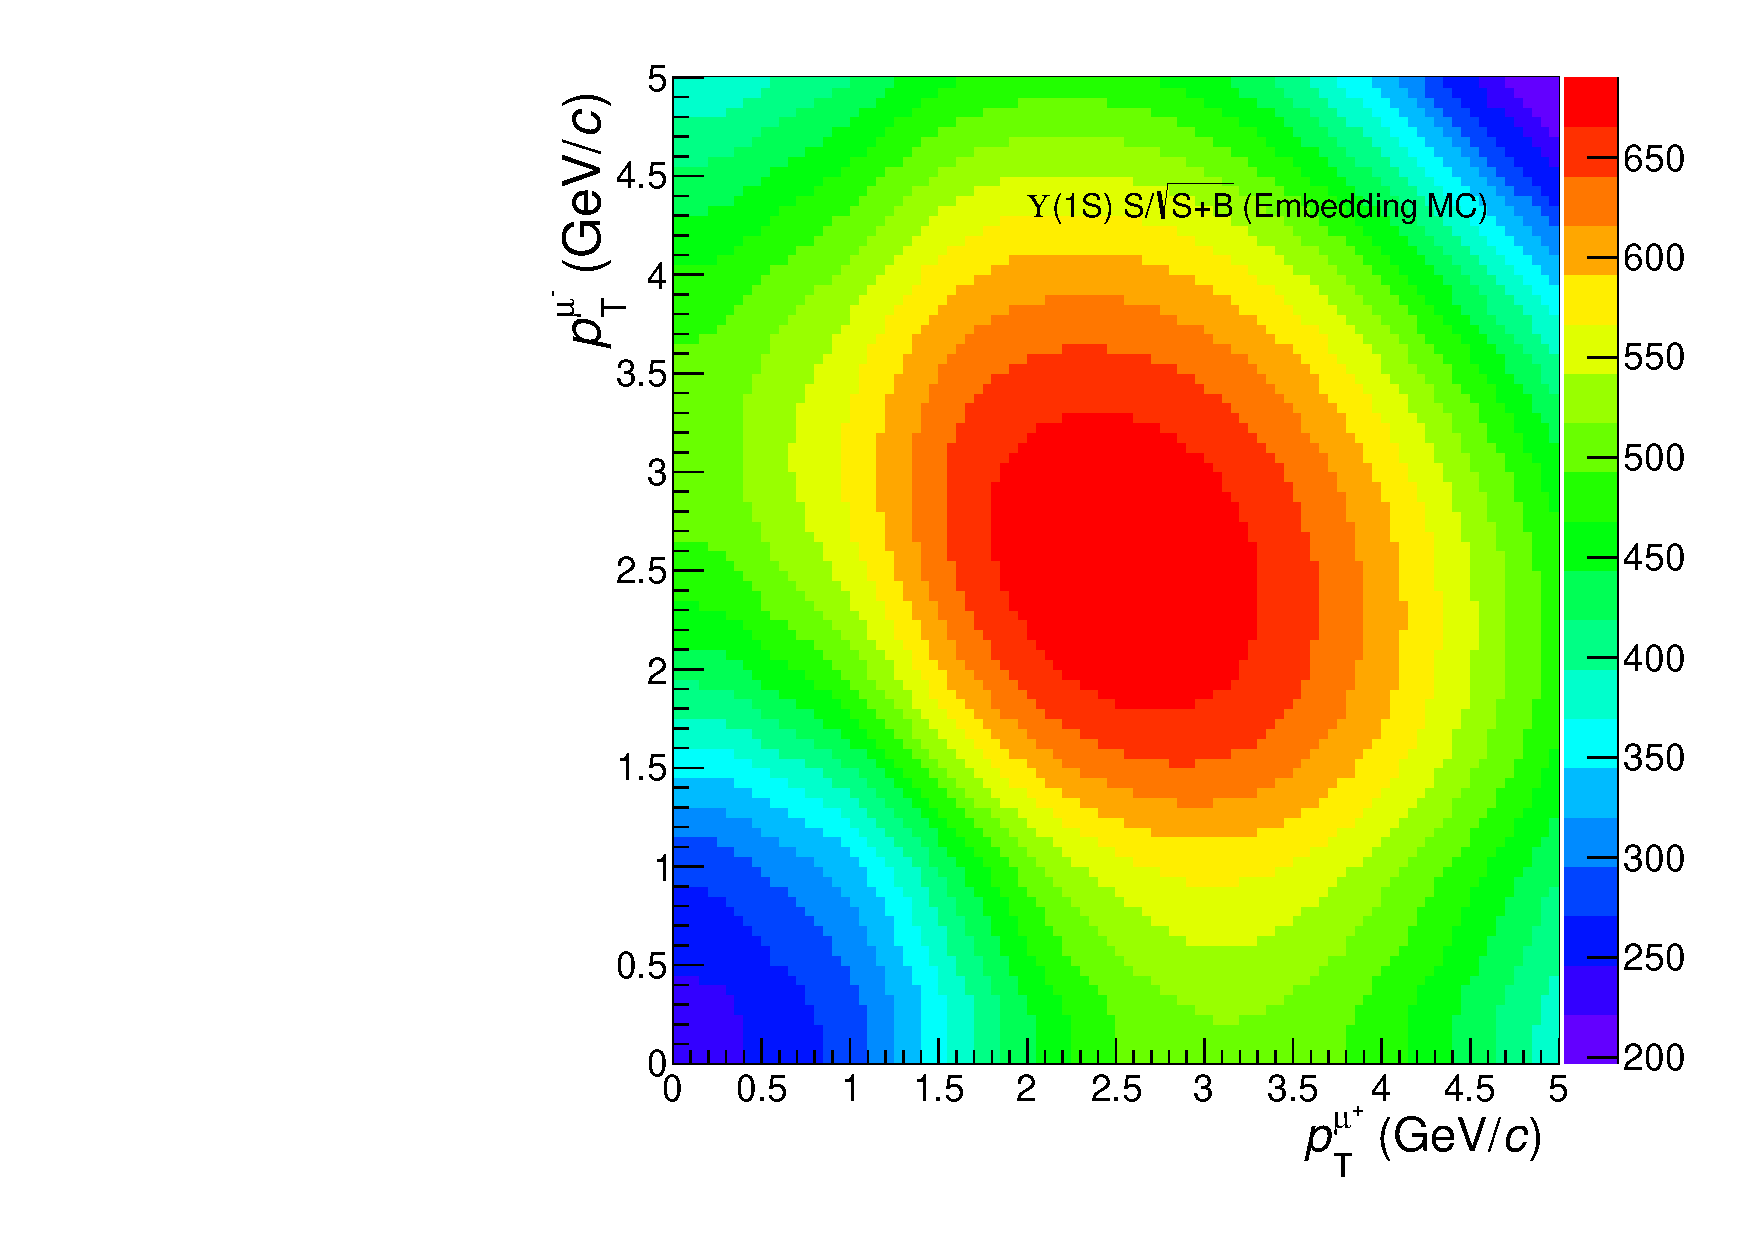
\includegraphics[width=6cm]{MuonPtCut/significance_rebin1_ptmax5_LinearScale.pdf}
\end{center}
\caption{\label{signifi}\ups significance as a function of the \pt cut of each muon computed from embedding MC.}
\end{figure}


\paragraph{Pair cuts}
\begin{itemize}
\item opposite charge
\item $-4<y<-2.5$
\item $\pt<12$
\end{itemize}

